\section{Projektorganisation}

Die Studierenden werden im Projekt 2 (pro2E) für den Studiengang Elektro- und Informationstechnik von fünf Dozenten der Fachhochschule Nordwestschweiz (FHNW) unterstützt. Pascal Buchschacher informiert über Projektmanagement allgemein, Anita Gertiser vermittelt den Studenten die richtige Kommunikation innerhalb des Teams und Peter Niklaus, Richard Gut  wie auch Sebastian Gaulocher steht als Ansprechpartner für Fragen technischer Natur zur Verfügung.
\subsection{Projektverantwortliche}

\subsection{Auftraggeber}
Auftraggeber des Projekts 2 ist Dr. Luca Dalessandro, Group Technology Manager der Schaffner Group.

\subsection{Teammitglieder}
Das Team 1 des Projekts 2 setzt sich aus sechs Studenten der Fachhochschule Nordwestschweiz, Hochschule für Technik in Brugg/Windisch zusammen. Niklaus Schwegler (NS) ist der Projektleiter und verantwortlich für die Arbeiten und die Kommunikation mit dem Auftraggeber und den Fachdozenten. Unterstützt wird dieser vom stellvertretenden Projektleiter \newline Marco  Binder (MB). Für die Ressort Software ist Pascal Puschmann (PP) und Elekrotechnik ist Lukas von Däniken (LD) zuständig. Die übrigen Mitglieder sind Simon Rohrer (SR) und Claudio Alfare (CA). Jeder von ihnen studiert Elektro- und Informationstechnik im zweiten Semester.

\subsection{Organigramm}
\begin{figure}[H]
	\centering
	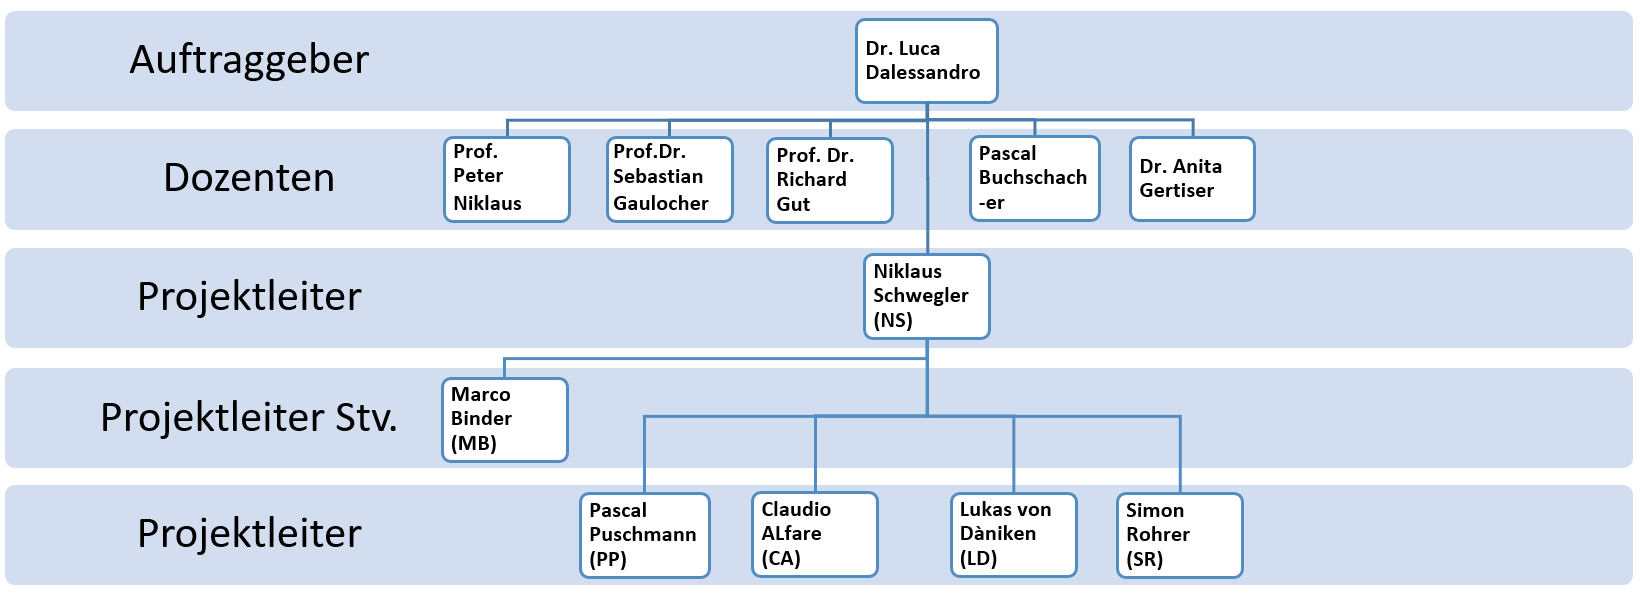
\includegraphics[width=10cm]{Organi.png}
	\label{fig:Organigramm}
\end{figure}
